\chapter{Intermolecular Forces}

\section{Dipole Moment and Polarization}

	Two equal and opposite charges separated by a certain distance constitute an \emph{electric dipole}. \\
	It is measured by the \emph{dipole moment} $\mathbf{\mu} = q\mathbf{d}$, whose unit is the Debye: $1\,\text{D} = 3.336\times 10^{-30}\,\text{C}\cdot\text{m}$. \\
	Molecules possessing a permanent dipole moment are called \emph{polar molecules}. \\\ \\
	%
	Under an external electric field, the orientation behavior of molecules is called \emph{polarization}.

	\subsection{Orientation Polarization}

		The energy of a dipole in an electric field is
		\[E(\theta) = -\mathbf{\mu}\cdot\mathbf{E} = -\mu E\cos\theta\]
		Therefore the molecule tends to align its own dipole moment with the field; this behavior is called \emph{orientation polarization}. \\\ \\
		%
		The distribution of the orientation angle $\theta$ obeys the Boltzmann distribution, so the probability of finding the dipole between $\theta$ and $\theta+\df\theta$ is
		\[\df p = \frac{e^{-\beta E(\theta)}\sin\theta\,\df\theta}{\displaystyle\int_{0}^{\pi}e^{-\beta E(\theta)}\sin\theta\,\df\theta}
		\qquad (E(\theta) = -\mu E\cos\theta)\]
		Then the expectation value of the dipole-moment component along the field direction, $\mu_z$, is
		\[\expect{\mu_z} = \int \mu\cos\theta\,\df p
		= \mu\,\frac{\displaystyle\int_{0}^{\pi}e^{x\cos\theta}\cos\theta\sin\theta\,\df\theta}
		{\displaystyle\int_{0}^{\pi}e^{x\cos\theta}\sin\theta\,\df\theta}
		\qquad \left(x = \frac{\mu E}{k_{\text{B}}T}\right)\]
		Substituting $y = \cos\theta$, the integrals can be carried out explicitly and one obtains
		\[\boxed{\expect{\mu_z} = \mu L(x), \quad
		L(x) = \frac{e^{x}+e^{-x}}{e^{x}-e^{-x}} - \frac{1}{x}}\]
		where $L(x)$ is called the \emph{Langevin function}. \\
		When $x \ll 1$, keeping the first term of the Taylor expansion $L(x) \approx x/3$ gives
		\[\boxed{\expect{\mu_z} = \frac{\mu^{2}E}{3k_{\text{B}}T}}\]
		i.e. the mean oriented dipole is proportional to the field and inversely proportional to the temperature.

	\subsection{Distortion and Electronic Polarization}\label{polarization}

		The electric field also distorts the positions of the nuclei within a molecule (\emph{distortion polarization}) and the distribution of the electrons (\emph{electronic polarization}). 
		The dipole moment thus produced (or modified) is called the \emph{induced dipole moment}, which is roughly proportional to the field strength:
		\[\mathbf{\mu}^{*} = \alpha\mathbf{E}, \qquad \alpha' = \frac{\alpha}{4\pi\varepsilon_0}\]
		The proportionality coefficient $\alpha$ is called the \emph{polarizability}; to simplify the units one also defines the \emph{polarizability volume} $\alpha'$.
		%
		\subsubsection{Relation between polarizability and structure.}
		Apply static perturbation theory with the perturbation
		\[\hat{H}^{(1)} = -\hat{\mu}_z E\]
		The second-order correction to the ground-state energy is
		\[E^{(2)} = \sum_{n}\frac{\left|\braket{\psi_0^{(0)}|\hat{H}^{(1)}|\psi_n^{(0)}}\right|^{2}}{E_0^{(0)}-E_n^{(0)}}
		= E^{2}\sum_{n}\frac{|\mu_{z,0n}|^{2}}{E_0^{(0)}-E_n^{(0)}}\]
		Meanwhile, as the field is increased from $0$ to $E$, the energy change of the induced dipole is
		\[\Delta E = -\int_{0}^{E}\mu^{*}\,\df E = -\frac{1}{2}\alpha E^{2}\]
		Comparing the two expressions one obtains
		\[\boxed{\alpha = 2\sum_{n}\frac{|\mu_{z,0n}|^{2}}{E_n^{(0)}-E_0^{(0)}}}\]
		%
		Denote the average excitation energy by $\Delta E$ (roughly the HOMO--LUMO gap), and take the most significant transition dipole to be of order $eR$; then
		\[\alpha \approx \frac{2e^{2}R^{2}}{\Delta E}\]
		That is, the larger the atom (molecule/ion) and the smaller the HOMO--LUMO gap, the more easily it is polarized. \\\ \\
		%
		Therefore in common ionic compounds, since the cation radius is smaller than the anion radius, the cation polarizes the anion, shifting the ionic bond towards covalency (generally results in lower melting point, water solubility and thermal instability). 
		The higher the charge and the smaller the radius of the cation, and the larger the radius and the higher the charge of the anion, the more pronounced the polarization (\emph{Fajans' rules}). \\ \\
		The polarization of $\rm CO_3^{2-}$ by metal cations weakens the C--O bond, making it easily decomposed.

	\subsection{The Vanishing of Polarization at High Frequencies}

		Since the rotation of a molecular dipole moment takes time (in fluids about $1\,\text{rad/ps}$), if the field direction changes too fast --- with frequency higher than $10^{11}\,\text{Hz}$ (microwave region) --- the molecules cannot respond in time and the orientation polarization vanishes. \\ \\
		Molecular vibration (displacement of the dipole) is the main principle of IR spectroscopy. When the frequency lies in the infrared region, the molecular vibration gradually fails to follow, so the distortion polarization gradually vanishes. 
		At still higher frequencies, only the electrons can respond in time, and only the electronic polarization remains.

\section{Van der Waals Interaction}

	A \emph{point dipole} is a dipole whose charge separation $l$ is much smaller than the observation distance $r$.

	\subsection{Dipole--Charge Interaction}

		For a point charge on the axis of a dipole with separation $l$, distance $r$ to its center, calculating the two dipole charges separately, the electrostatic potential energy is
		\[V = -\frac{1}{4\pi\varepsilon_0}\left(\frac{q_1 q_2}{r-\frac{l}{2}} - \frac{q_1 q_2}{r+\frac{l}{2}}\right)
		= -\frac{q_1 q_2}{4\pi\varepsilon_0\,r}\left(\frac{1}{1-x} - \frac{1}{1+x}\right)\]
		where $x = l/2r \ll 1$ (point dipole). Expanding through the geometric (Taylor) series
		\[V = -\frac{q_1 q_2}{4\pi\varepsilon_0\,r}\left[\left(1+x+x^{2}+x^{3}+\cdots\right) - \left(1-x+x^{2}-x^{3}+\cdots\right)\right]\]
		and discarding the higher-order terms, the point-dipole--charge interaction is obtained:
		\[\boxed{V = -\frac{\mu_1 q_2}{4\pi\varepsilon_0\,r^{2}}}\]
		Notice that the decay is $1/r^{2}$ rather than $1/r$ as between two charges: viewed from a large scale, the dipole's charges cancel each other. \\ \\
		For interactions between higher multipoles, the decay is $1/r^{\,n+m+1}$ (for a $2^n$-pole and a $2^m$-pole).

	\subsection{Dipole--Dipole Interaction}
		
		Let the displacement from the center of the dipole to the test charge $\mathbf{r}$, 
		the distance to the $\pm$ charge of the dipole $r_{\pm}$. The dipole potential can be written as
		\[V(\mathbf{r}) = \frac{1}{4\pi\varepsilon_0}\left(\frac{q}{r_+} - \frac{q}{r_-}\right)\]
		By the law of cosines, discarding the tiny terms (since for a point dipole $r \gg d$, $d/r \ll 1$):
		\[r_{\pm}^{2} = r^{2} + \left(\frac{d}{2}\right)^{2} \mp rd\cos\theta
		= r^{2}\left(1 \mp \frac{d}{r}\cos\theta + \frac{d^{2}}{4r^{2}}\right)
		\approx r^{2}\left(1 \mp \frac{d}{r}\cos\theta\right)\]
		Since $d/r$ is also tiny, expanding $(1\pm x)^{-1/2} = 1 \mp x/2$ at $x = 0$ gives
		\[\frac{1}{r_{\pm}} = \frac{1}{r}\left(1 \mp \frac{d}{r}\cos\theta\right)^{-1/2}
		\approx \frac{1}{r}\left(1 \pm \frac{d}{2r}\cos\theta\right)
		\ \Rightarrow\ 
		\frac{1}{r_+} - \frac{1}{r_-} = \frac{d}{r^{2}}\cos\theta\]
		Hence the dipole potential (with $\mu = qd$):
		\[\boxed{V_{\text{dip}}(\mathbf{r}) = \frac{\mu\cos\theta}{4\pi\varepsilon_0 r^{2}} = \frac{\mathbf{\mu}\cdot\hat{\mathbf{r}}}{4\pi\varepsilon_0 r^{2}}}\]\\
		%
		The electric field is the negative gradient of the potential, $\mathbf{E}_{\text{dip}}(\mathbf{r}) = -\nabla V_{\text{dip}}(\mathbf{r})$:
		\[\frac{\partial}{\partial r}V(\mathbf{r}) = \frac{-2\mu\cos\theta}{4\pi\varepsilon_0 r^{3}}, \qquad
		\frac{1}{r}\frac{\partial}{\partial\theta}V(\mathbf{r}) = \frac{-\mu\sin\theta}{4\pi\varepsilon_0 r^{3}}
		\quad (\text{no } \varphi \text{ part})\]
		giving the dipole field in spherical coordinates:
		\[\mathbf{E}_{\text{dip}}(\mathbf{r}) = \frac{\mu}{4\pi\varepsilon_0 r^{3}}\left(2\cos\theta\,\hat{\mathbf{r}} + \sin\theta\,\hat{\boldsymbol{\theta}}\right)\]
		A coordinate transformation then yields a frame-independent expression. Placing the dipole on the $z$-axis, $\mathbf{\mu} = \mu\hat{\mathbf{z}}$, and using
		$\hat{\mathbf{z}} = \cos\theta\,\hat{\mathbf{r}} - \sin\theta\,\hat{\boldsymbol{\theta}}$, one finds
		\[2\cos\theta\,\hat{\mathbf{r}} + \sin\theta\,\hat{\boldsymbol{\theta}}
		= 3\cos\theta\,\hat{\mathbf{r}} - \left(\cos\theta\,\hat{\mathbf{r}} - \sin\theta\,\hat{\boldsymbol{\theta}}\right)
		= 3(\hat{\mathbf{z}}\cdot\hat{\mathbf{r}})\hat{\mathbf{r}} - \hat{\mathbf{z}}\]
		Hence the coordinate-free dipole field:
		\[\boxed{\mathbf{E}_{\text{dip}}(\mathbf{r}) = \frac{1}{4\pi\varepsilon_0 r^{3}}\left(3(\mathbf{\mu}\cdot\hat{\mathbf{r}})\hat{\mathbf{r}} - \mathbf{\mu}\right)}\]\\
%
		For two parallel dipoles held in parallel to each other with displacement $\mathbf{r}$, let $\theta=\expect{\mu,\mathbf{r}}$, 
		the potential energy is
		\[V = -\mathbf{E}_1\cdot\mathbf{\mu}_2 = \frac{\mu_1\mu_2\,f(\theta)}{4\pi\varepsilon_0 r^{3}}, \qquad f(\theta) = 1 - 3\cos^{2}\theta\]
		If they could rotate completely freely, $\expect{f} = 0$ and hence $\expect{V} = 0$. \\ \\
		But in reality the rotation is not completely free: due to the Boltzmann distribution the low-energy orientations are preferred, so $\expect{f}$ acquires a probability weighting
		\[\expect{f} = \expect{f}_0\,e^{-V/k_{\text{B}}T} = \expect{f}_0 - \frac{V}{k_{\text{B}}T}\expect{f^{2}}_0 + \cdots\]
		Since $\expect{f}_0 = 0$ and The average value $\expect{f^2}_0$ turns out to be 2/3 when the calculation is carried through in
detail over all orientations but not only when they're parallel, keeping up to the quadratic term gives the \emph{Keesom interaction}:
		\[\boxed{\expect{V} = -\frac{2\mu_1^{2}\mu_2^{2}}{3(4\pi\varepsilon_0)^{2}\,k_{\text{B}}T\,r^{6}}}\]
		Inversely proportional to the sixth power of the distance indicates this is a van der Waals force; the negative sign indicates attraction, with an energy of roughly $-0.07\,\text{kJ}\cdot\text{mol}^{-1}$. \\\ \\

	\subsection{Dipole--Induced Dipole Interaction}

		The dipole field of a polar molecule induces an induced dipole in another molecule (proportional to the field strength, i.e. proportional to $r^{-3}$). 
		The two dipoles then interact; as their directions are consistent, the average does not vanish (the interaction of parallel dipoles is proportional to $r^{-3}$):
		\[\boxed{V = -\expect{\mathbf{\mu}^{*}\cdot\mathbf{E}} = -\frac{\mu_1^{2}\,\alpha_2'}{4\pi\varepsilon_0\,r^{6}}}\]
		This \emph{Debye induction interaction} is again a $r^{-6}$ van der Waals attraction.

	\subsection{Transient Dipole--Induced Dipole Interaction}

		A nonpolar molecule produces an \emph{instantaneous (transient) dipole} due to the instantaneous uneven distribution of its electron cloud.
		This dipole in turn induces an induced dipole in a neighboring molecule; the two share the same direction, so the average is not zero. \\\ \\
		%
		The ability of a molecule to produce a transient dipole is negatively related to its ability to bind its electrons (the ionization energy $I$): the weaker the binding, the more the electron cloud fluctuates, and the larger the probability of an instantaneously uneven distribution, the more easily a transient dipole arises. \\ \\
		The ability to produce an induced dipole is likewise negatively related to the electron-binding ability (the polarizability $\alpha'$).
		%
		Therefore the dispersion force is well approximated by the \emph{London dispersion formula}:
		\[\boxed{V = -\frac{3\,I_1 I_2\,\alpha_1'\alpha_2'}{2(I_1+I_2)\,r^{6}}}\]

\section{Exchange Repulsion}\label{exchange}

	When two closed-shell molecules approach so closely that their electron clouds overlap, the Pauli exclusion principle requires different orbitals remain orthogonal, and thus forces the electrons into smaller spaces with higher-energy states, producing a strong short-range \emph{exchange repulsion}. 
	Unlike the power-law attractive terms above, the exchange repulsion decays \emph{exponentially} with the overlap of the wavefunctions:
	\[V_{\text{rep}}(r) = A\,e^{-Br}\]
	It is commonly approximated by a steep power law $B'/r^{12}$. Combined with the $r^{-6}$ van der Waals attraction, the total interaction is modeled by the \emph{Lennard-Jones potential}:
	\[\boxed{V(r) = 4\epsilon\left[\left(\frac{\sigma}{r}\right)^{12} - \left(\frac{\sigma}{r}\right)^{6}\right]}\]
	with a minimum $V = -\epsilon$ at the equilibrium distance $r_{\text{eq}} = 2^{1/6}\sigma$, which defines the sum of the van der Waals radii. \\\ \\
	%
	Exchange repulsion is present in \emph{every} intermolecular interaction discussed below; it sets the closest contact distance and balances the attractive electrostatic, induction and dispersion terms.
\section{Hydrogen Bond and Halogen Bond}
\subsection{Hydrogen Bond}\label{hbond}

	An ordinary \emph{hydrogen bond} is the attraction $\text{X}-\text{H}\cdots\text{Y}$ between two molecules, where X and Y are highly electronegative and Y bears a lone pair; among them N, O and F participate in hydrogen bonding most effectively, while $sp^2,\ sp$ C and Si can also participate. \\
	As an interaction of $\sim 20\,\text{kJ}\cdot\text{mol}^{-1}$, its energy makes it dominant among intermolecular forces.

	\subsubsection{Electrostatic Attraction}

		A hydrogen bond can be viewed as the electrostatic attraction of Y's lone pair towards the exposed hydrogen nucleus: the highly electronegative X drains the electron density of H, leaving it positively charged and its nucleus poorly shielded, which then attracts the electron cloud of Y. In order to reduce electrostatic repulsion of negatively charged X and Y, the ideal configuration of hydrogen bond is linear.\\ \\
		Due to the dual attraction from both X and Y, the hydrogen is even more electron deficient, $\delta$ generally shifts downfield.
		This is the dominant force in hydrogen bond interaction.

	\subsubsection{Charge Transfer and Rehybridization}
		Combining the $\sigma$ and $\sigma^*$ orbital of X--H and the lone-pair orbital $n$ of Y gives three three-center orbitals --- bonding, nonbonding and antibonding --- occupied by four electrons (figure \ref{3c4e}); this is the three-center four-electron (3c-4e) bond.
		\begin{figure}[h]
			\centering
			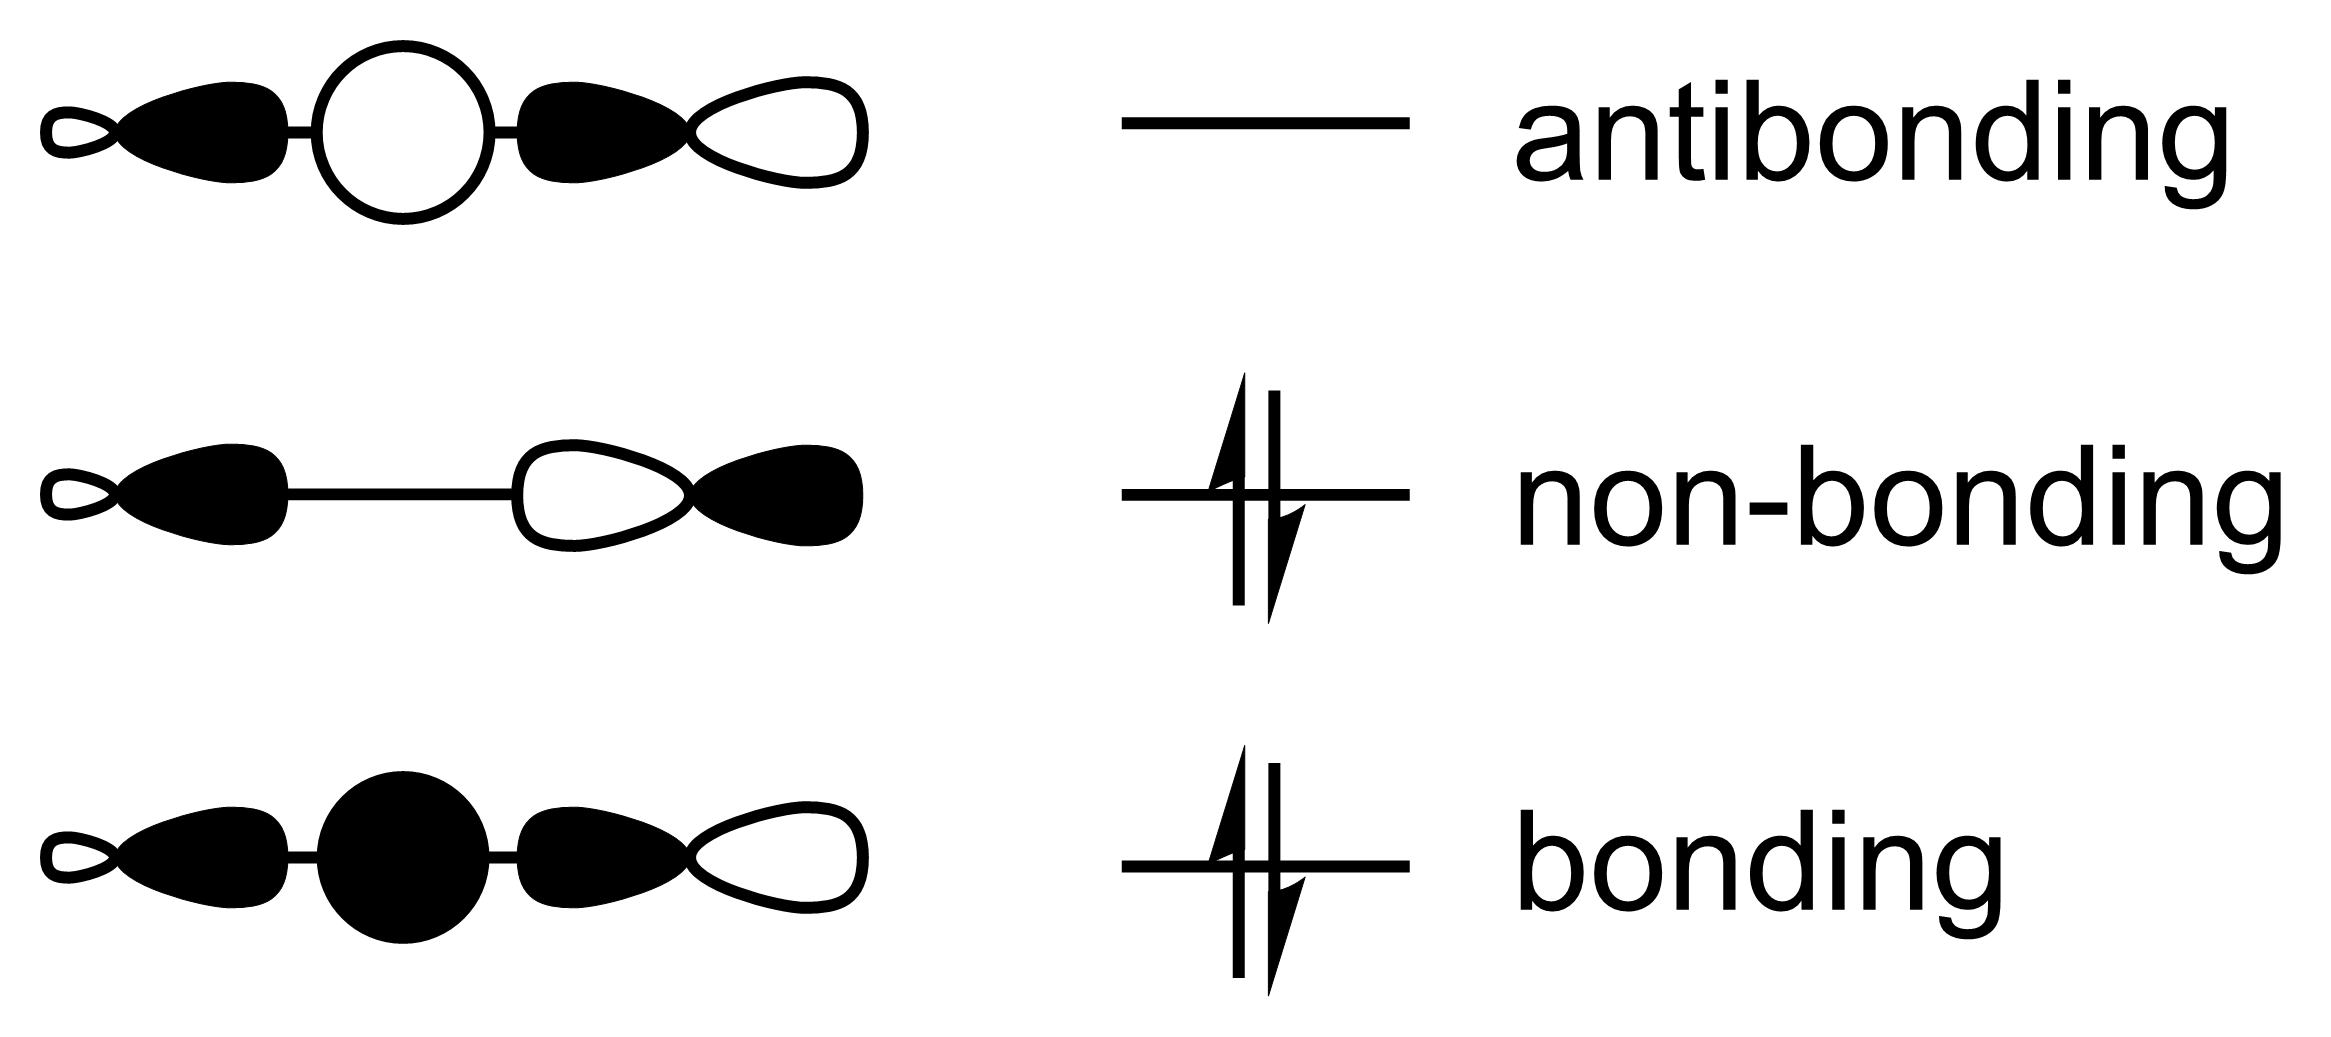
\includegraphics[scale=0.1]{Ch8/hb}
			\caption{Three-center four-electron molecular orbitals of a hydrogen bond}
			\label{3c4e}
		\end{figure}\ \\
		An equivalent description is the \emph{hyperconjugation} (charge transfer) from the lone pair of Y into the antibonding orbital of X--H, $n_{\text{Y}} \to \sigma^{*}_{\text{XH}}$: the donor--acceptor mixing transfers electron density from Y to the X--H unit, stabilizing the complex and weakening and lengthening the X--H bond. \\ \\
		The filling of antibonding orbital polarized X--H towards X even more, 
		leading to an increased electron density in X's orbital. 
		According to Bent's rule, X will use more $s$ component to bond with H, which in turn strengthened X--H bond.
		This rehybridization effect is significant to those prone to hybridize, like C.\\ \\
		Consequently two classes appear, named after the change in IR spectroscopy (vibration wavenumber $\tilde{\nu}$) of the X--H bond:
		\begin{itemize}
			\item Red-shifted (proper) hydrogen bonds: the $n_{\text{Y}} \to \sigma^{*}_{\text{XH}}$ charge transfer populates the antibonding orbital, X--H lengthens and its stretching frequency decreases (e.g. O--H$\cdots$O).
			\item Blue-shifted (improper) hydrogen bonds: when rehybridization dominates over the $\sigma^{*}$ population, X--H contracts and its stretching frequency increases (e.g. some C--H$\cdots$O bonds).
		\end{itemize}

	\subsubsection{Induction and Exchange Repulsion}

		The mutual polarization of the donor and acceptor also contributes; it is especially important in \emph{weak} hydrogen bonds where charge transfer is small. Exchange repulsion between the closed shells of X and Y counteracts the attraction and sets the $\text{H}\cdots\text{Y}$ contact distance.
		\begin{figure}[h]
		\centering
		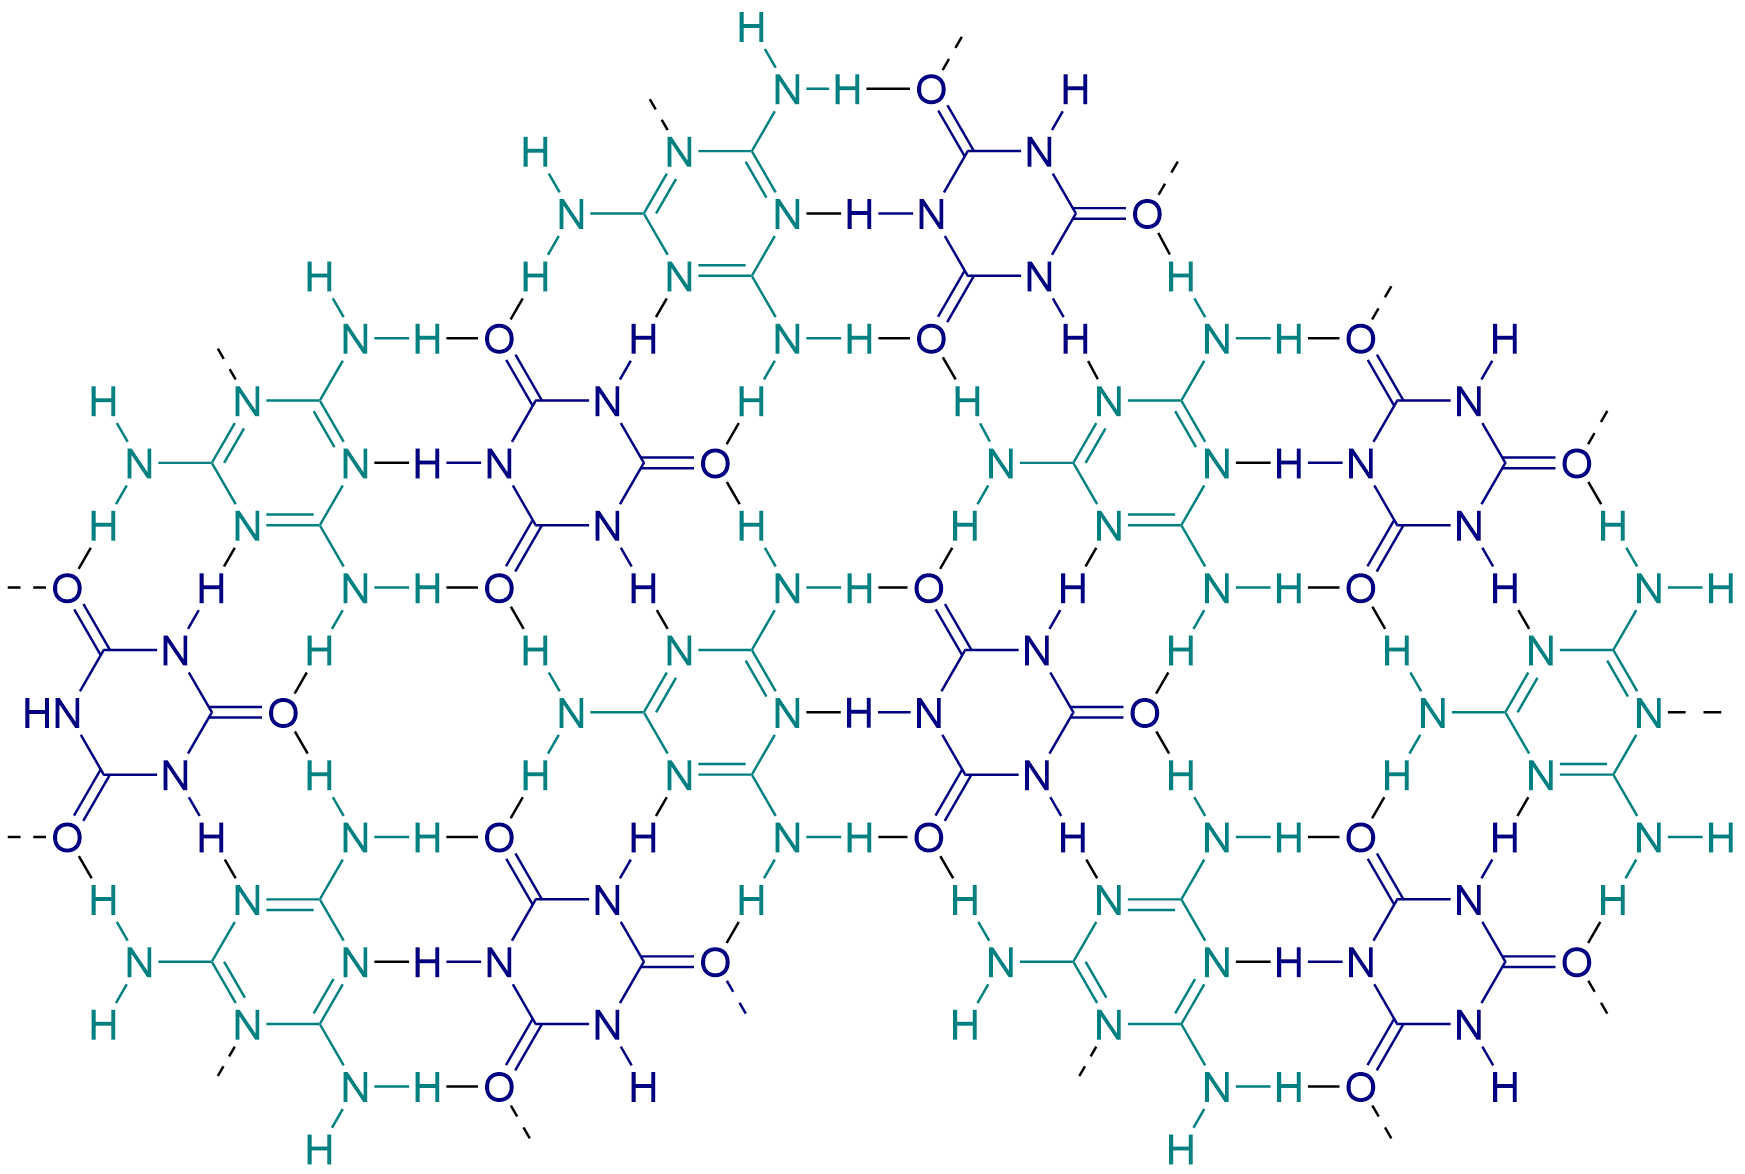
\includegraphics[scale=0.2]{Ch8/HBnetwork}
		\caption{Hydrogen bonded supramolecule of melamine and cyanuric acid}
		\end{figure}

	\subsubsection{Symmetric and Unusual Hydrogen Bonds}

		Except in $\rm HF_2^-$, where $\text{F}-\text{H}\cdots\text{F}^- \leftrightarrow \text{F}^-\cdots\text{H}-\text{F}$ is a \emph{symmetric hydrogen bond}, in general A---H is shorter than $\text{H}\cdots\text{B}$. \\ \\
		Electron-rich conjugated systems (aromatic $\pi$ clouds) and even metals can also act as hydrogen-bond acceptors.
		In aromatic hydrogen bonds, due to the shielding of $\pi$ clouds, hydrogen $\delta$ may shift upfield. \\\ \\
		In $\text{A}-\text{H}\cdots\text{H}-\text{B}$, where A--H is protonic and B--H hydridic, a \emph{dihydrogen bond} forms between the two hydrogens, as in ammonia borane $\rm H_3N\!\to\!BH_3$.

\subsection{Halogen Bond}\label{xbond}

	A \emph{halogen bond} is the attraction $\text{R}-\text{X}\cdots\text{Y}$ between a covalently bound halogen X and a Lewis base Y, despite both being nominally negatively charged.

	\subsubsection{Electrostatic Origin: the $\sigma$-Hole}
		The bonding electron density of X is polarized toward the R---X bond axis, while the electron cloud perpendicular to the axis remains roughly spherical; this leaves a region of positive electrostatic potential on X along the extension of the bond, which attracts the lone pair of Y (figure \ref{sigmahole}).
		\begin{figure}[h]
			\centering
			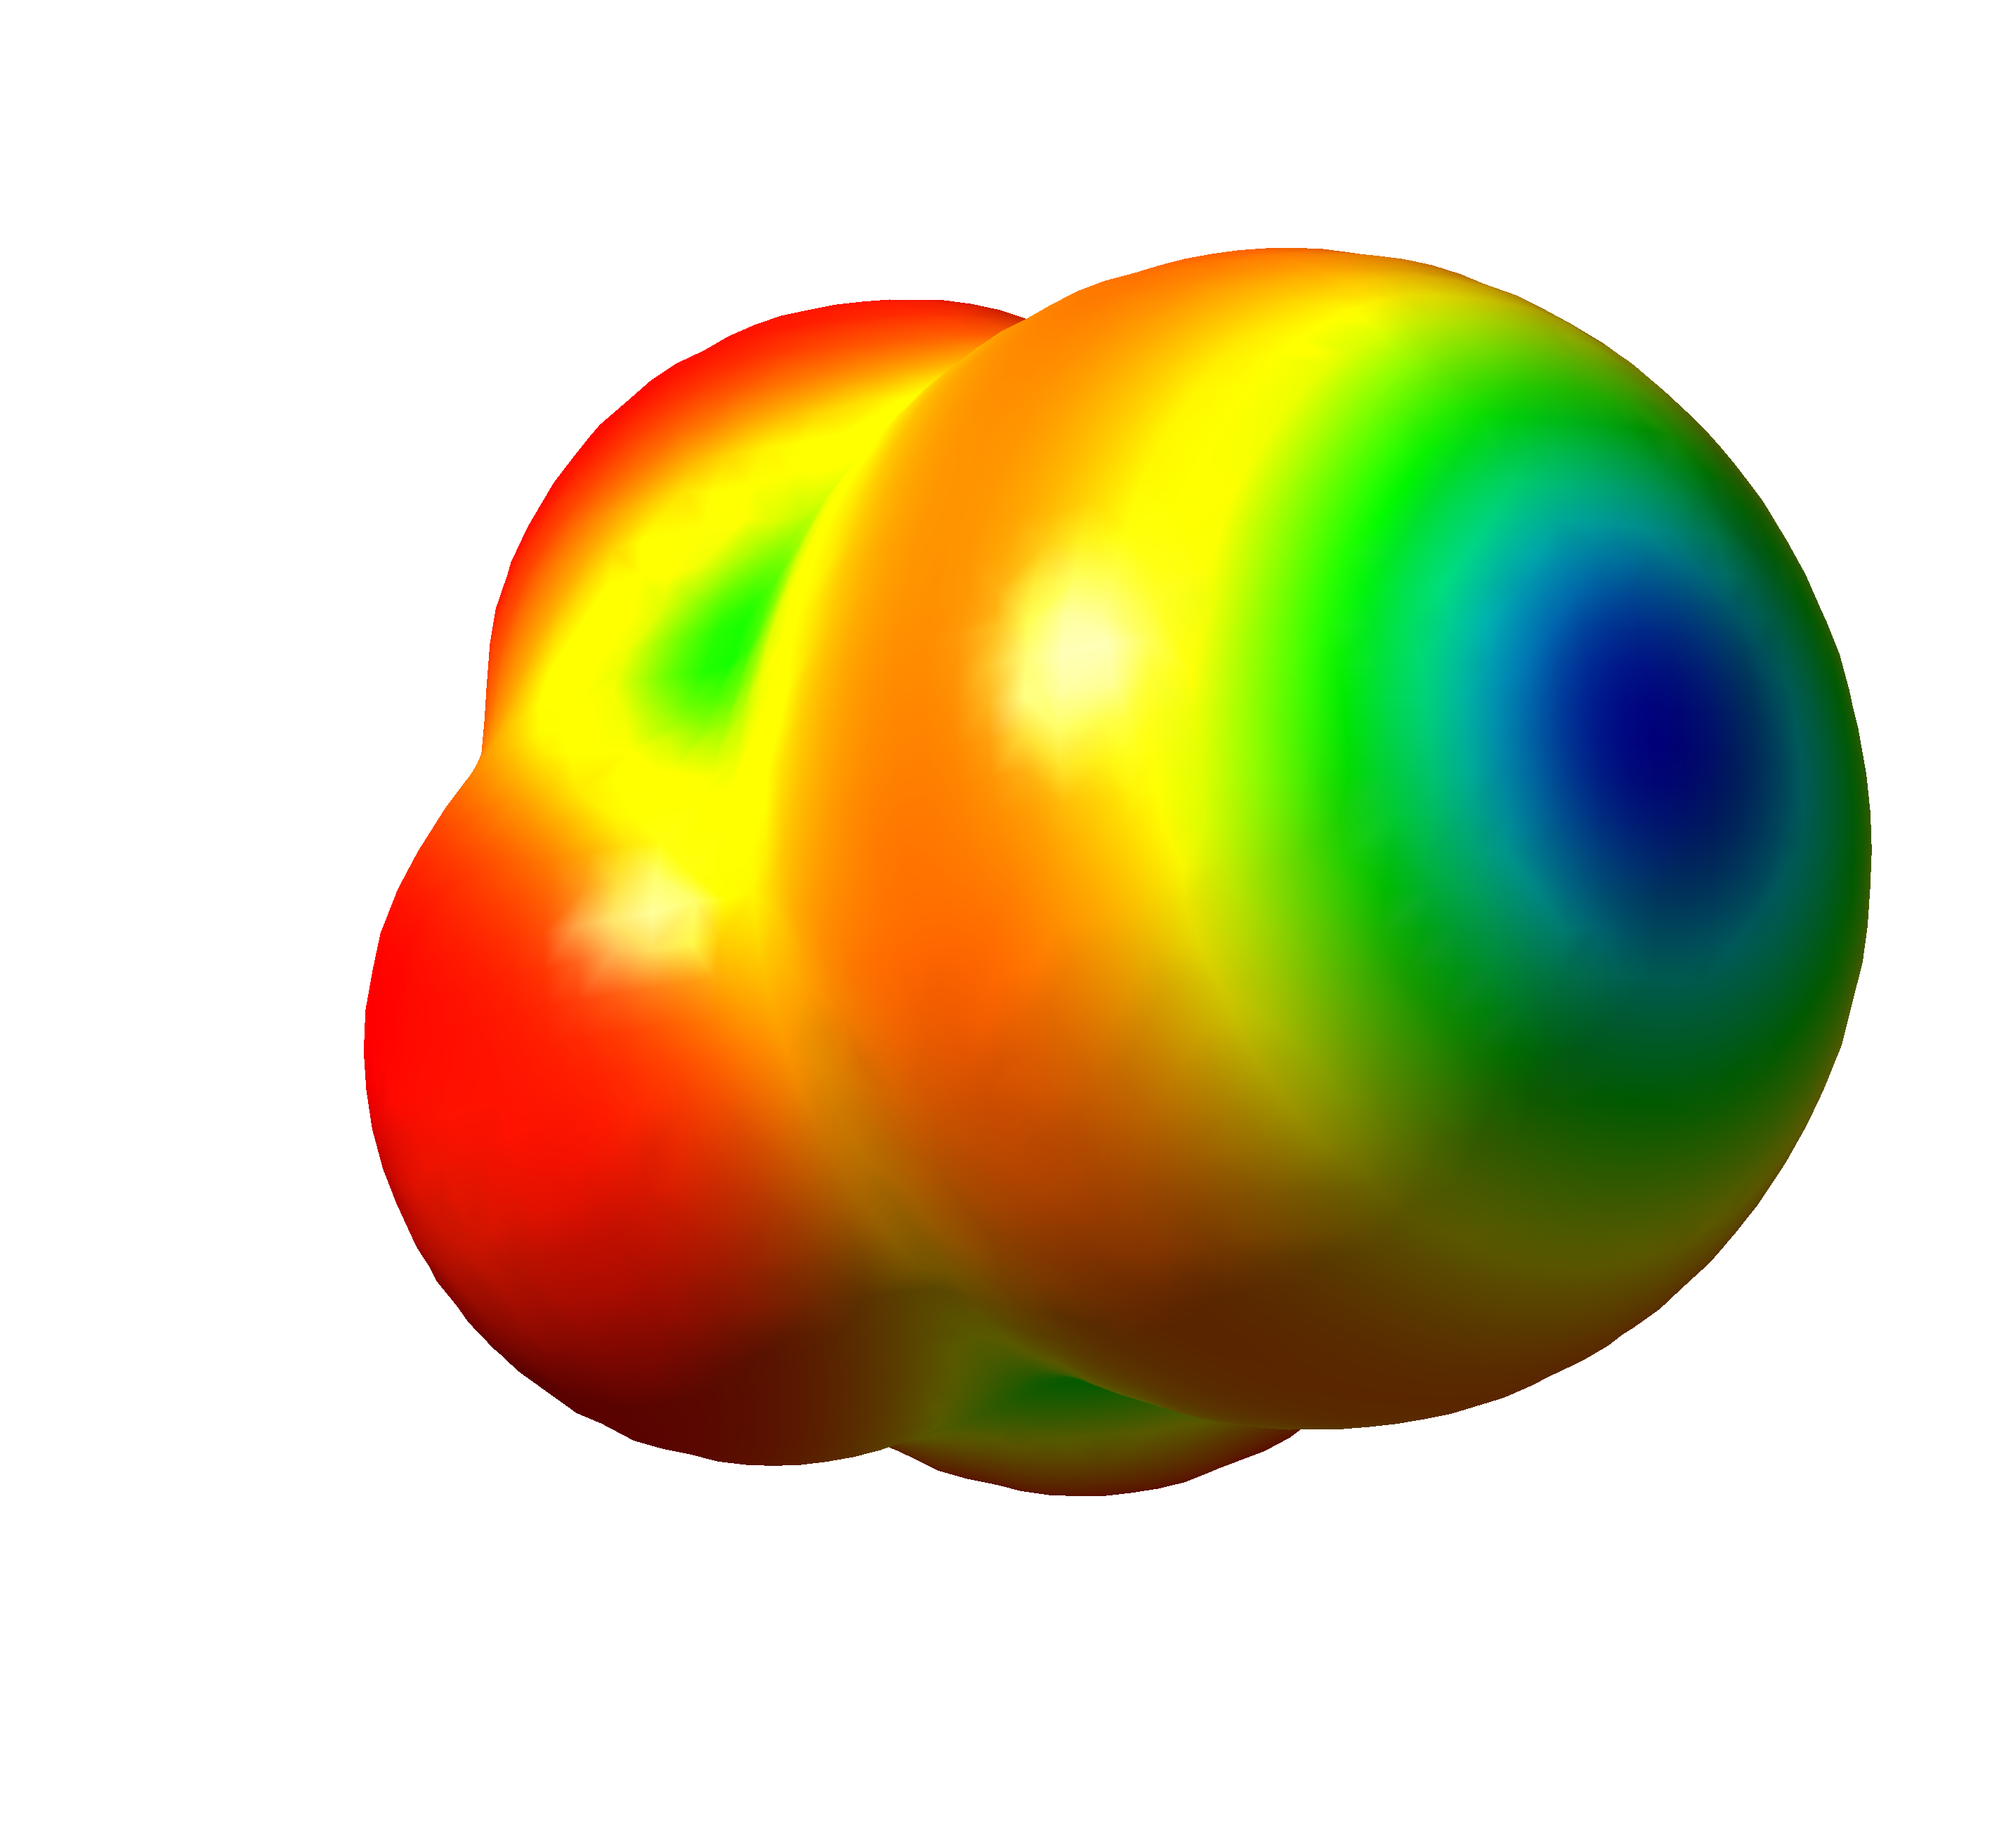
\includegraphics[scale=0.08]{Ch8/sh1}
			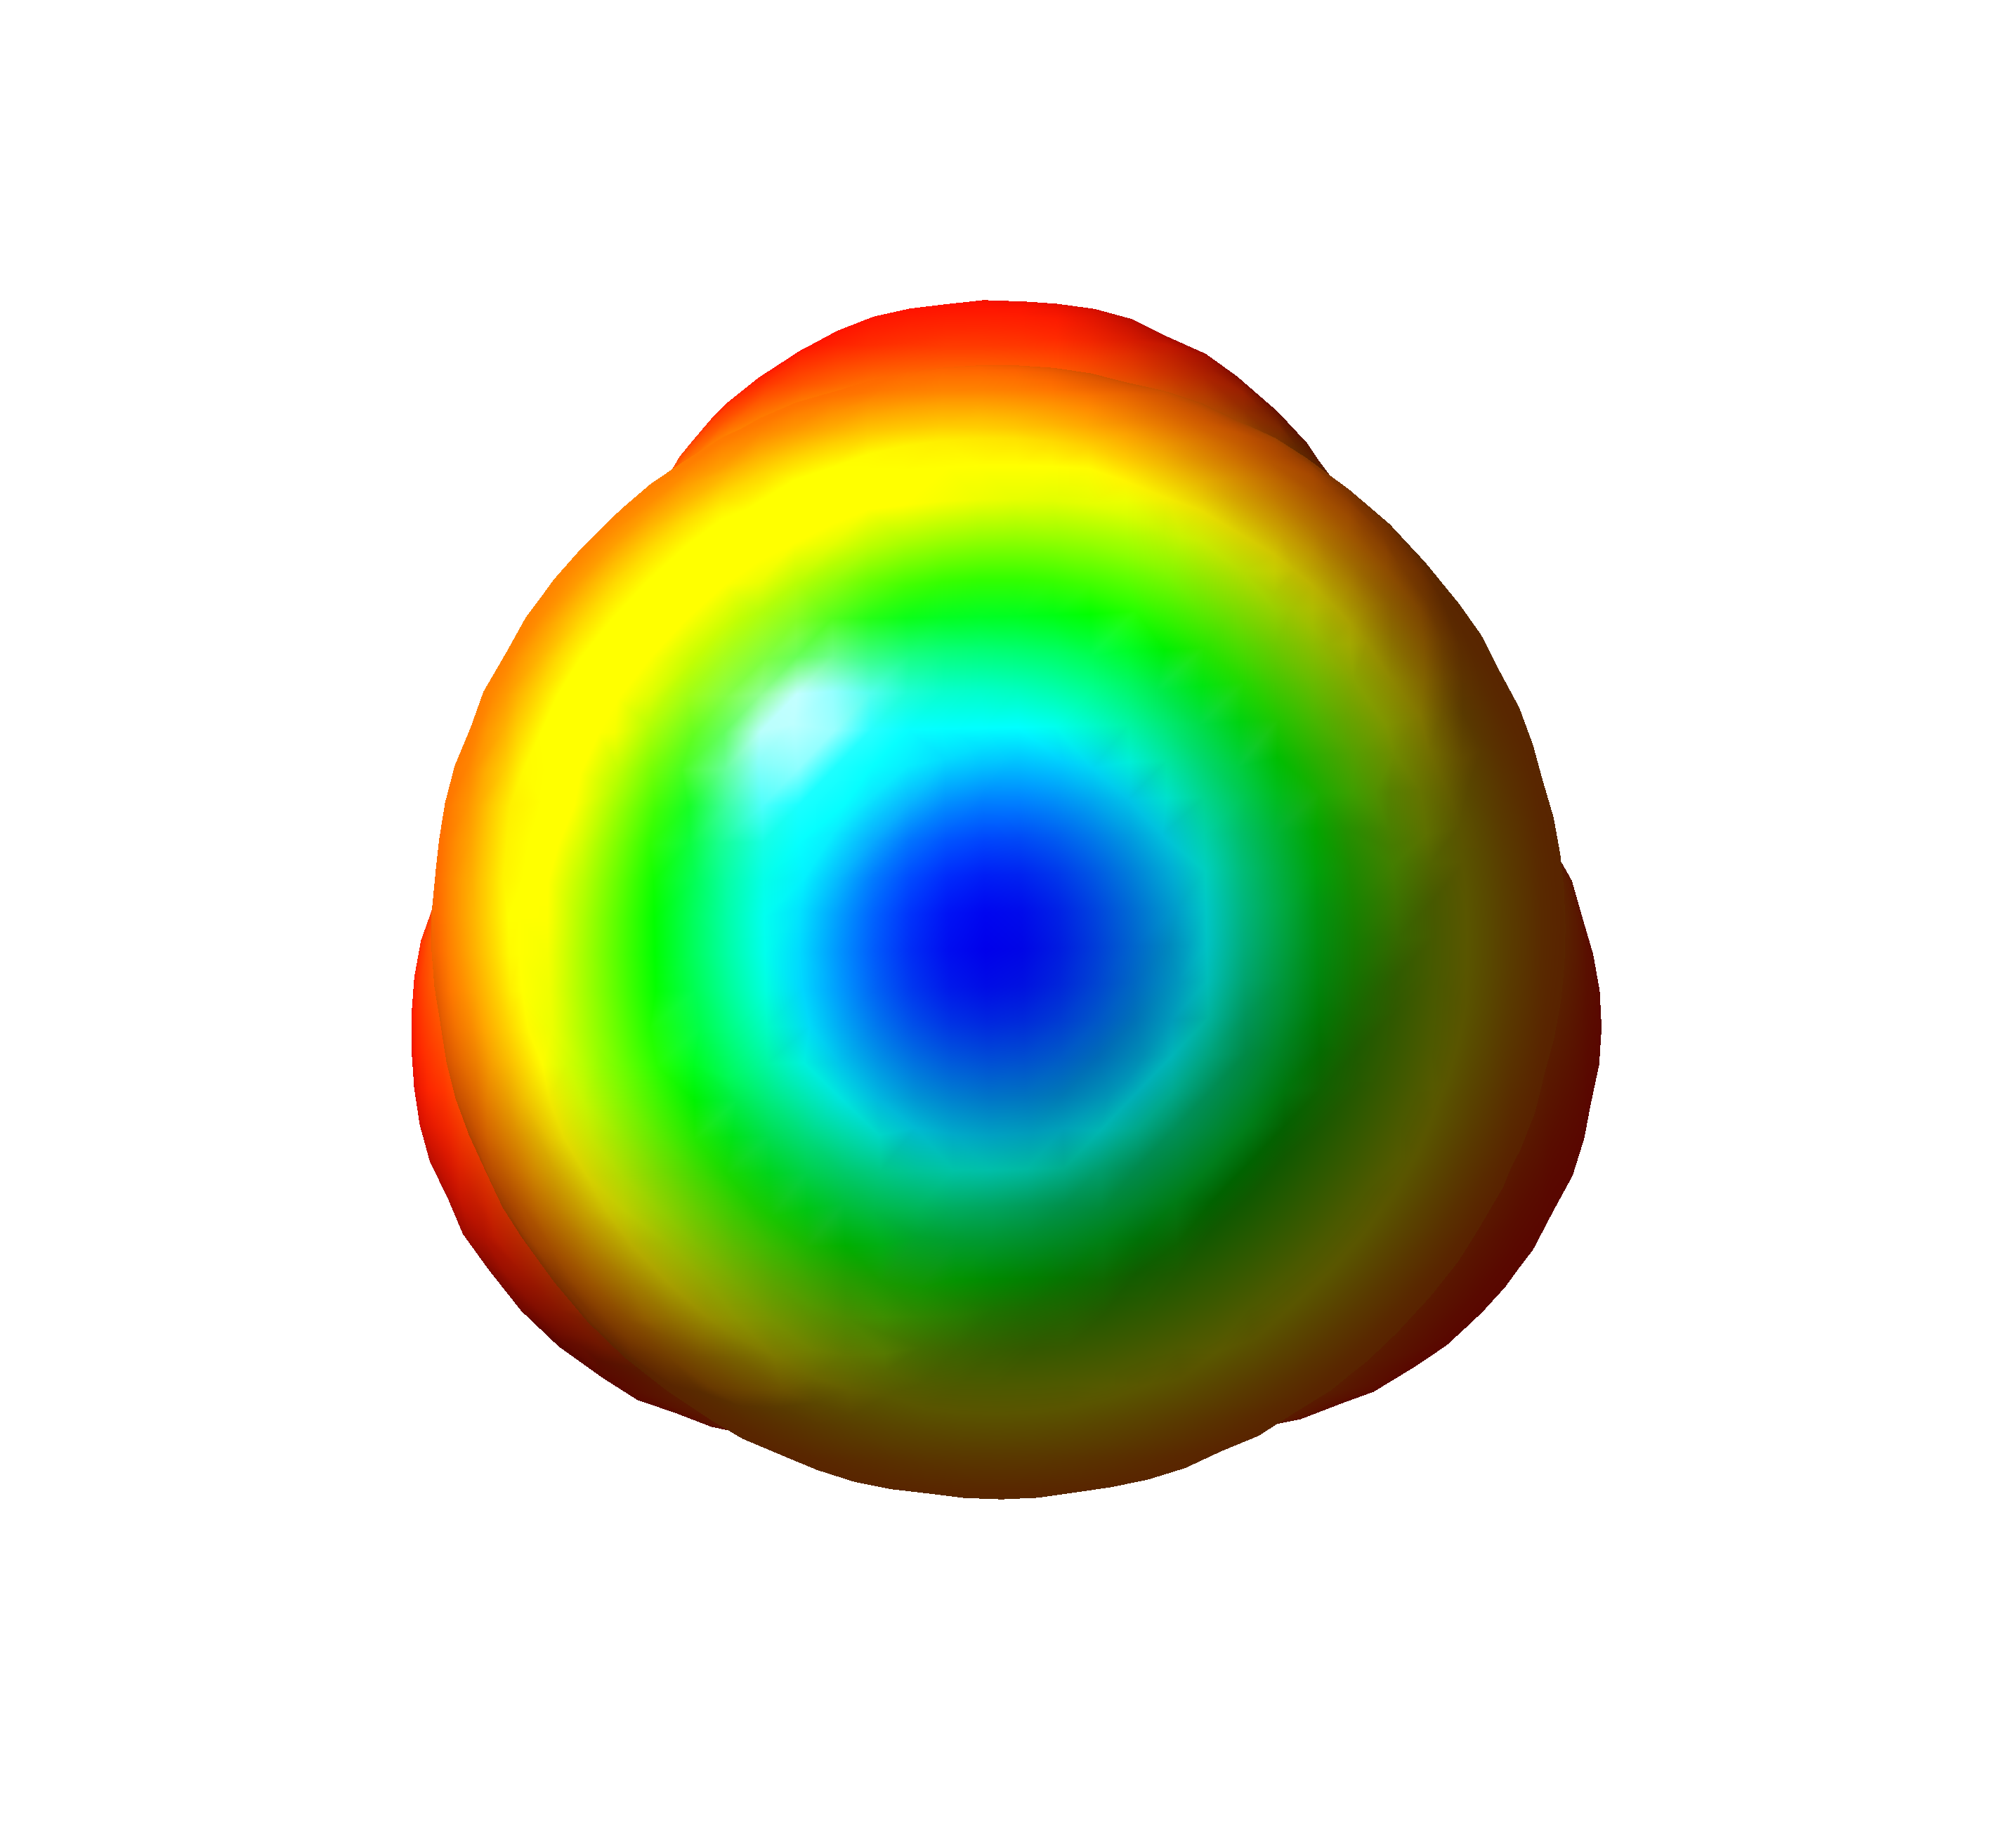
\includegraphics[scale=0.08]{Ch8/sh2}
			\caption{The surface electrostatic potential diagram of trifluoroiodomethane}
			\label{sigmahole}
		\end{figure}\ \\
		The more polarizable the halogen ($\text{I} > \text{Br} > \text{Cl} \gg \text{F}$) and the more electronegative the substituent R, the deeper the $\sigma$-hole and the stronger the halogen bond, thus alkynyl iodine and iodine cyanide are among the best halogen bond donors.\\ \\
		%
		Unlike hydrogen bond, the configuration of halogen bond can be either linear in the case of lone pair--$\sigma$ hole attraction, 
		or bent when two hole--lone pair system pairs up and dimerize. This polymerization is verified by electronic microscopy.
		\begin{figure}[h]
			\centering
			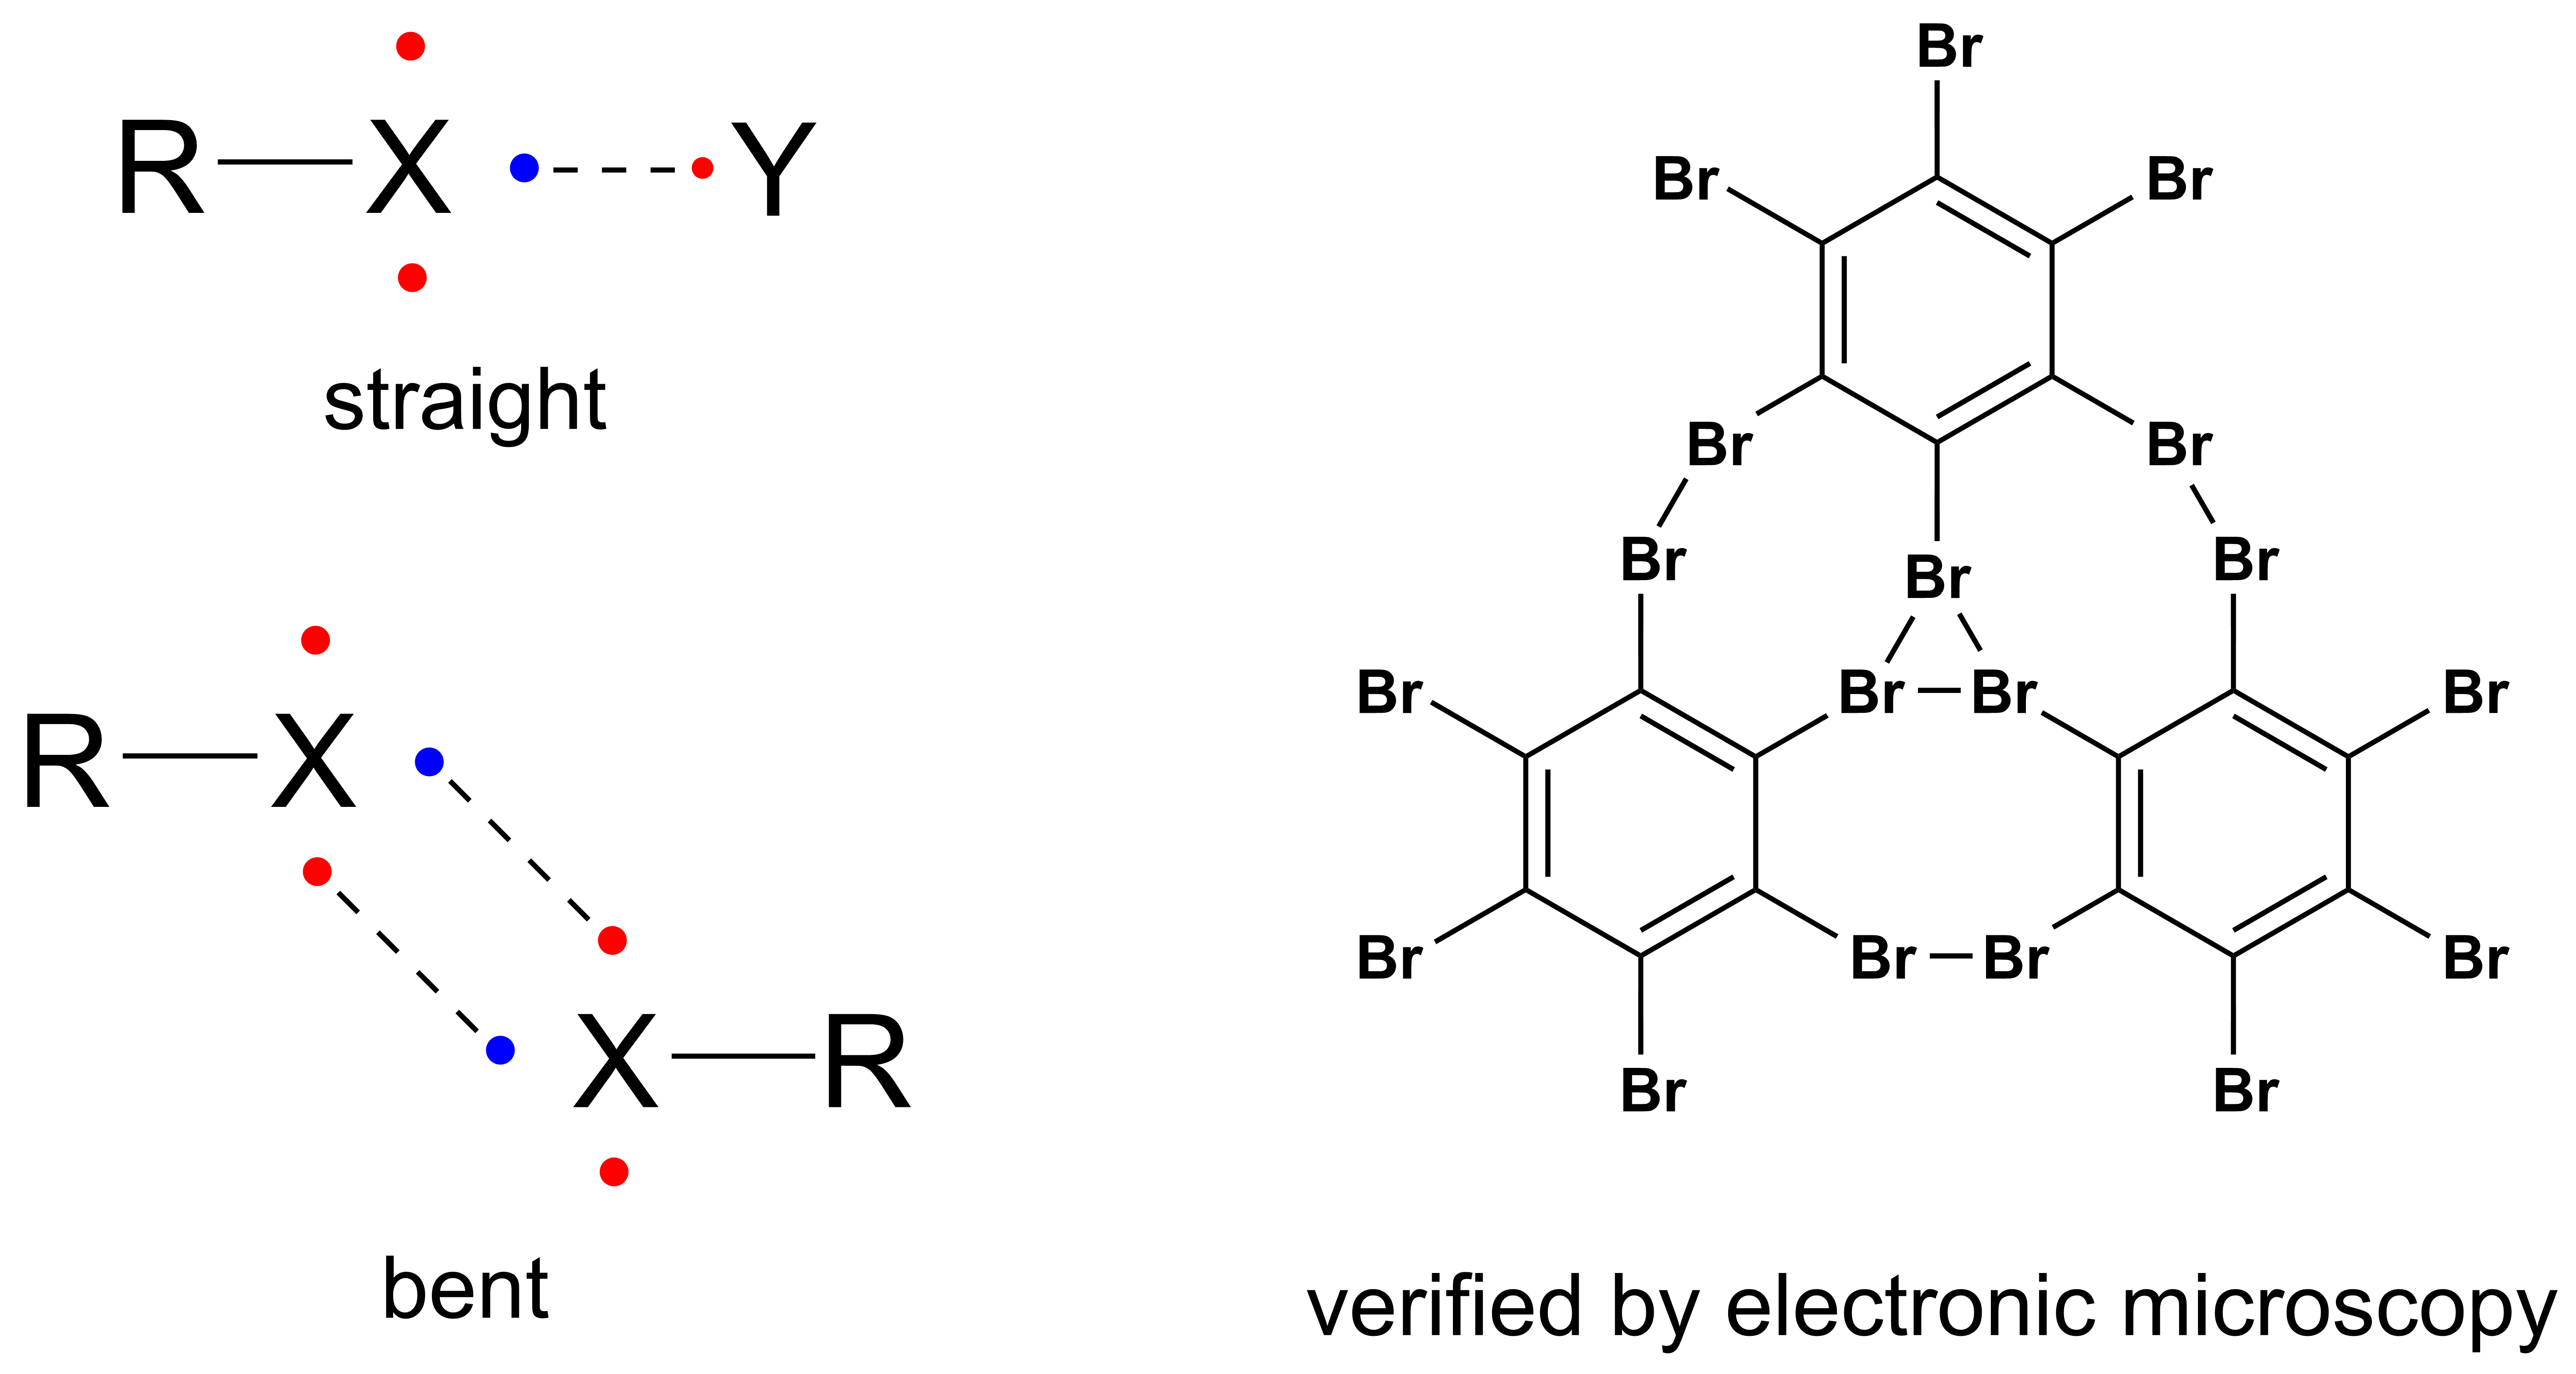
\includegraphics[scale=0.05]{Ch8/xb}
			\caption{The configuration of halogen bond}
		\end{figure}\ \\
		This configuration is also seen in crystalline halogens and multiatomic halogen ions (e.g. I$_2$ and I$_3^-$).

	\subsubsection{Charge Transfer, Induction, Dispersion and Exchange Repulsion}

		As in the hydrogen bond, there is charge transfer $n_{\text{Y}} \to \sigma^{*}_{\text{RX}}$. 
		For halogens of higher periods the radial overlap is poorer and the $\sigma^{*}_{\text{RX}}$ level lies lower, 
		so the charge transfer is stronger, another reason why heavier halogens bond more strongly. 
		As heavy halogens are softer, this orbital interaction plays a bigger role in halogen bond than in hydrogen bond. \\ \\
		%
		The formation of charge transfer complex also gives account to 
		why iodine takes on a brown color in polar solvents while remaining purple in nonpolar ones, 
		as $n_{\text{Y}} \to \sigma^{*}_{\text{RX}}$ raises the LUMO of the complex, 
		leading to a blue shift in UV-Vis absorption peak.\\ \\
		%
		The large, well-polarizable electron cloud of the halogen also 
		makes van der Waals induction and dispersion contributions significant, 
		while exchange repulsion again limits the contact distance.
		
		\subsection{Hydrogen Bond Enhanced Halogen Bond}
		The co-effect of hydrogen bond and halogen bond may lead to a stronger interaction. As in the following example, 
		\begin{itemize}
		\item The H on the benzene forces the amide coplanar with the ring via hydrogen bond while simultaneously polarizes carbonyl towards O even more, making the H--N more electron deficient and enhances H--I hydrogen bond;
		\item H--I hydrogen bond polarize the electron cloud off iodine perpendicular to C--I bond, which helps the formation of $\sigma$ hole.
		\end{itemize}
		\begin{figure}[h]
			\centering
			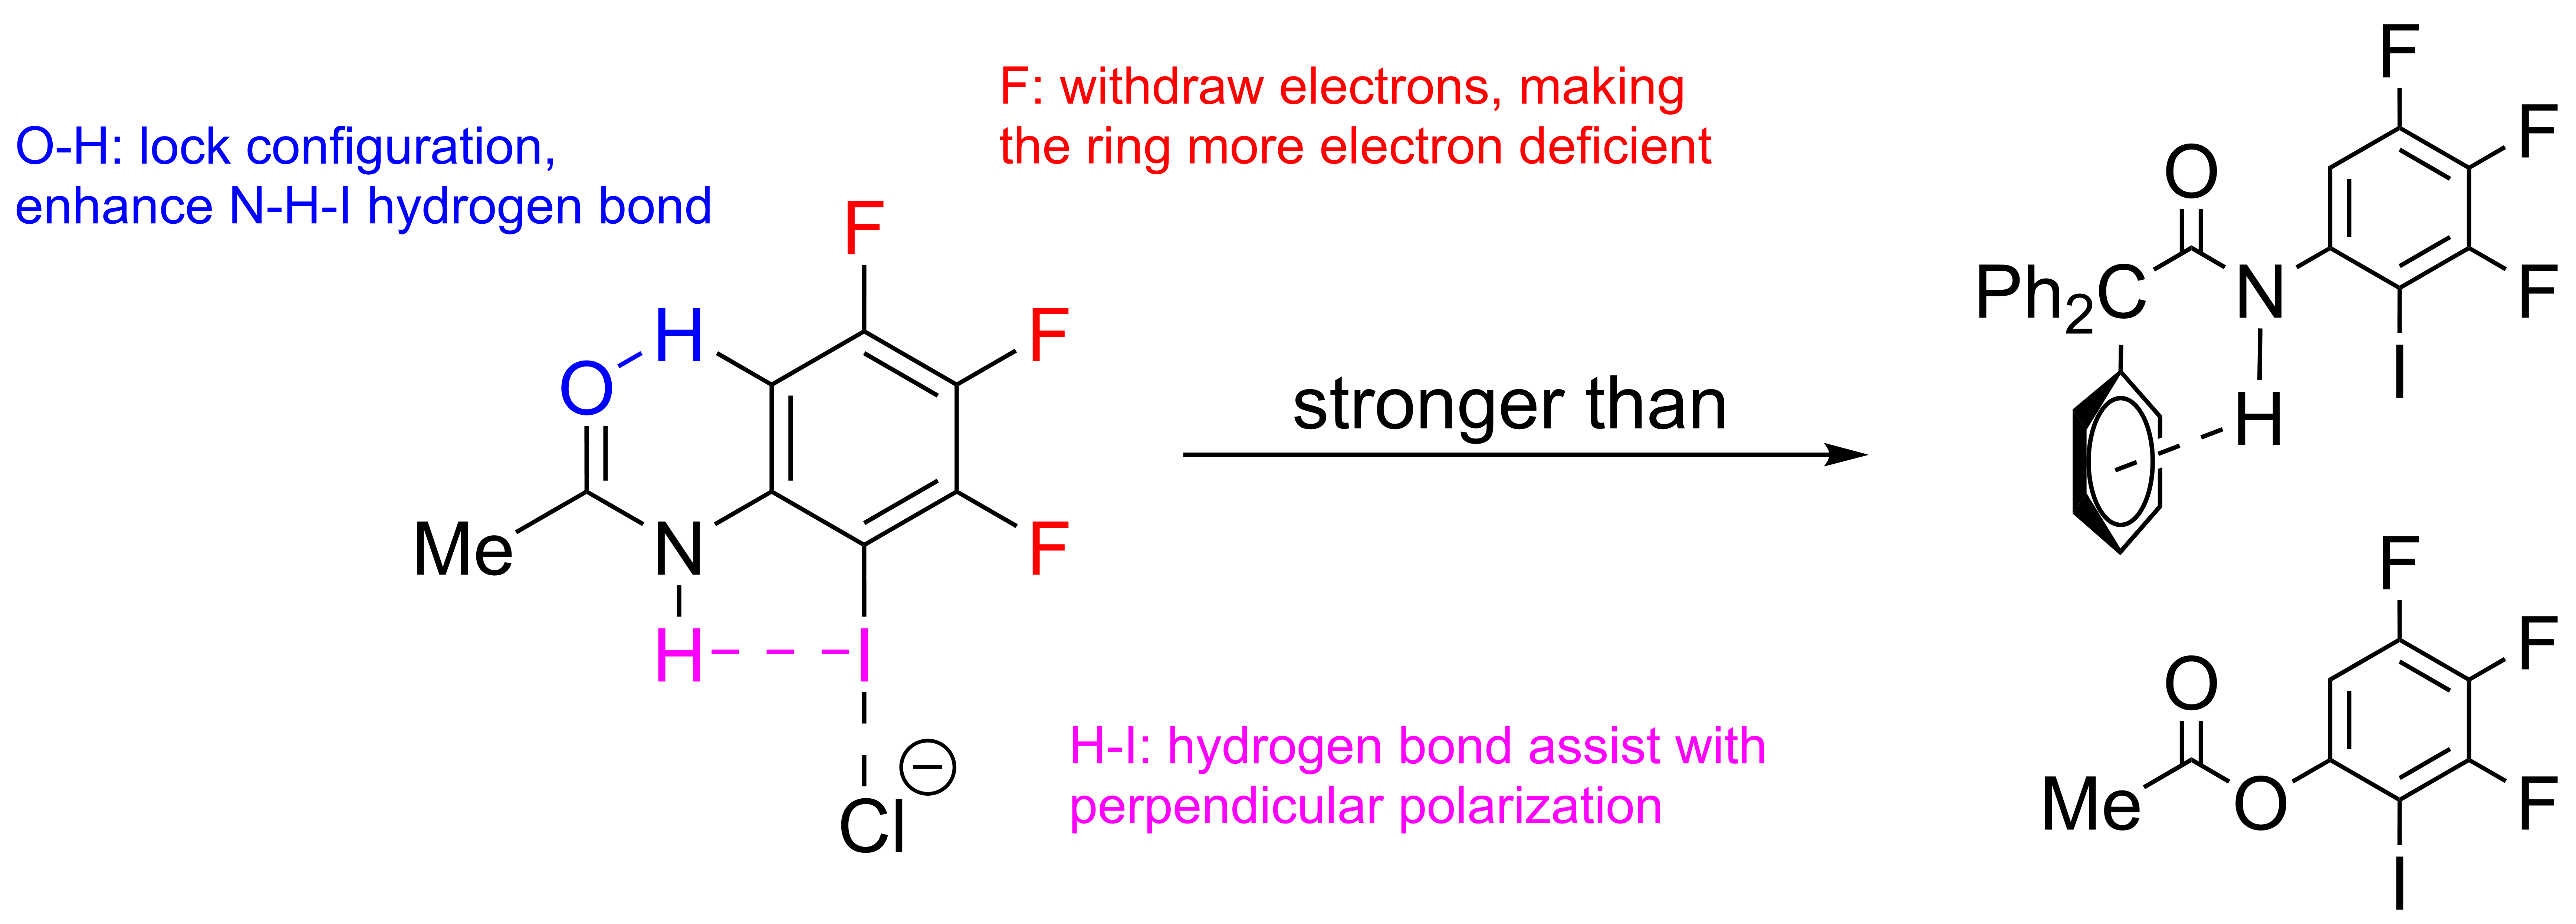
\includegraphics[scale=0.06]{Ch8/hbexb}
			\caption{Hydrogen bond enhanced halogen bond}
		\end{figure}
\section{$\pi$--$\pi$ Stacking}\label{pistack}

	\subsubsection{Configurations}
		Aromatic rings stack in three characteristic configurations (figure \ref{stackconf}): \emph{parallel} (sandwich), \emph{parallel-displaced} (glided) and \emph{perpendicular} (T-shaped) stacking.
		\begin{figure}[h]
			\centering
			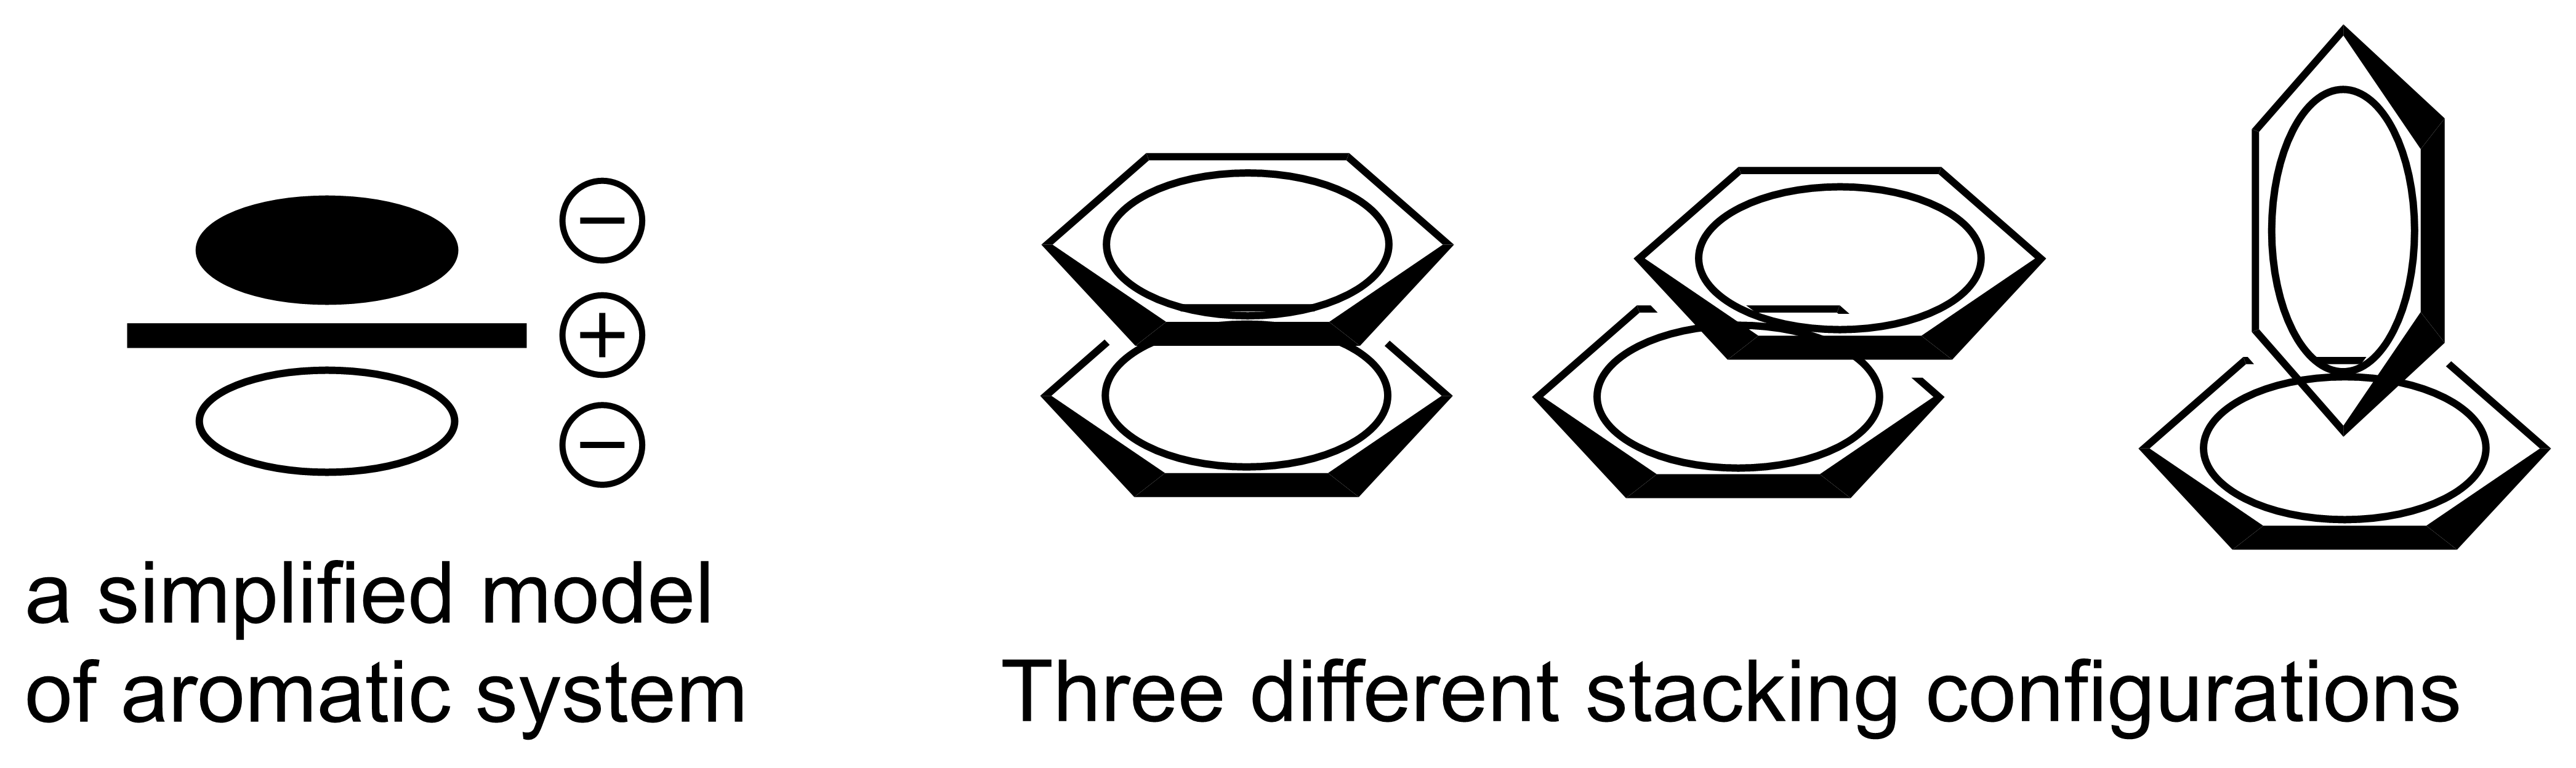
\includegraphics[scale=0.08]{Ch8/stack}
			\caption{Configurations of $\pi$--$\pi$ stacking}
			\label{stackconf}
		\end{figure}

	\subsubsection{Physical Origins}

		Each benzene ring carries a quadrupole moment with a negative $\pi$ cloud above and below the plane and a positive rim of C---H bonds. When the rings come close, \emph{quadrupole charge penetration} turns the naive quadrupole--quadrupole repulsion of the sandwich geometry into attraction (the electron clouds interpenetrate), and the T-shaped and displaced geometries place the positive rim of one ring against the negative face of the other. \\ \\
		The aromatic $\pi$ electron cloud is highly polarizable, so dispersion contributes strongly; the stacked rings are close in distance, where exchange repulsion balances the attraction. In solution, \emph{desolvation} of the contact faces further drives the stacking.

	\subsubsection{Substituent Effects}

		Substituents influence stacking mainly through their \emph{dipole (direct electrostatic) effect} on the local charge distribution of the ring, rather than by globally enriching or depleting the $\pi$ cloud. \\
		When one ring is electron rich and the other electron deficient, \emph{charge transfer} from the former to the latter additionally stabilizes the stack, as in charge-transfer complexes.

\section{Hydrophobic Interaction}\label{hydrophobic}

	If the transfer of a species from a nonpolar solvent into a polar solvent is not spontaneous, i.e. $\Delta G > 0$, the species is called \emph{hydrophobic}. \\
	The hydrophobicity is measured by the \emph{hydrophobic constant} (for a group R, comparing the oil/water partition of RA and HA):
	\[\pi = \log P_{\text{RA}} - \log P_{\text{HA}}, \qquad P = \frac{S_{\text{oct}}}{S_{\text{water}}}\]
	where $P$ is the octanol--water partition coefficient, the ratio of solubilities in the two phases. \\\ \\
	%
	Its essence: each nonpolar solute molecule forces the surrounding water to form an ordered solvent cage (losing entropy); the aggregation of nonpolar molecules into an `oil drop' reduces the total cage surface, releasing the caged water. The increase of the water's entropy drives the aggregation --- an entropy-driven ordering process.
